% Options for packages loaded elsewhere
\PassOptionsToPackage{unicode}{hyperref}
\PassOptionsToPackage{hyphens}{url}
%
\documentclass[
  a4paper,
]{article}
\usepackage{amsmath,amssymb}
\usepackage{setspace}
\usepackage{iftex}
\ifPDFTeX
  \usepackage[T1]{fontenc}
  \usepackage[utf8]{inputenc}
  \usepackage{textcomp} % provide euro and other symbols
\else % if luatex or xetex
  \usepackage{unicode-math} % this also loads fontspec
  \defaultfontfeatures{Scale=MatchLowercase}
  \defaultfontfeatures[\rmfamily]{Ligatures=TeX,Scale=1}
\fi
\usepackage{lmodern}
\ifPDFTeX\else
  % xetex/luatex font selection
\fi
% Use upquote if available, for straight quotes in verbatim environments
\IfFileExists{upquote.sty}{\usepackage{upquote}}{}
\IfFileExists{microtype.sty}{% use microtype if available
  \usepackage[]{microtype}
  \UseMicrotypeSet[protrusion]{basicmath} % disable protrusion for tt fonts
}{}
\makeatletter
\@ifundefined{KOMAClassName}{% if non-KOMA class
  \IfFileExists{parskip.sty}{%
    \usepackage{parskip}
  }{% else
    \setlength{\parindent}{0pt}
    \setlength{\parskip}{6pt plus 2pt minus 1pt}}
}{% if KOMA class
  \KOMAoptions{parskip=half}}
\makeatother
\usepackage{xcolor}
\usepackage[margin=1in]{geometry}
\usepackage{graphicx}
\makeatletter
\def\maxwidth{\ifdim\Gin@nat@width>\linewidth\linewidth\else\Gin@nat@width\fi}
\def\maxheight{\ifdim\Gin@nat@height>\textheight\textheight\else\Gin@nat@height\fi}
\makeatother
% Scale images if necessary, so that they will not overflow the page
% margins by default, and it is still possible to overwrite the defaults
% using explicit options in \includegraphics[width, height, ...]{}
\setkeys{Gin}{width=\maxwidth,height=\maxheight,keepaspectratio}
% Set default figure placement to htbp
\makeatletter
\def\fps@figure{htbp}
\makeatother
\setlength{\emergencystretch}{3em} % prevent overfull lines
\providecommand{\tightlist}{%
  \setlength{\itemsep}{0pt}\setlength{\parskip}{0pt}}
\setcounter{secnumdepth}{-\maxdimen} % remove section numbering
\ifLuaTeX
\usepackage[bidi=basic]{babel}
\else
\usepackage[bidi=default]{babel}
\fi
\babelprovide[main,import]{catalan}
% get rid of language-specific shorthands (see #6817):
\let\LanguageShortHands\languageshorthands
\def\languageshorthands#1{}
\ifLuaTeX
  \usepackage{selnolig}  % disable illegal ligatures
\fi
\usepackage{bookmark}
\IfFileExists{xurl.sty}{\usepackage{xurl}}{} % add URL line breaks if available
\urlstyle{same}
\hypersetup{
  pdftitle={U1. Introducció als sistemes operatius en xarxa (I)},
  pdfauthor={@tofermos 2024},
  pdflang={ca-ES},
  hidelinks,
  pdfcreator={LaTeX via pandoc}}

\title{U1. Introducció als sistemes operatius en xarxa (I)}
\author{@tofermos 2024}
\date{}

\begin{document}
\maketitle

{
\setcounter{tocdepth}{2}
\tableofcontents
}
\setstretch{1.5}
\newpage
\renewcommand\tablename{Tabla}

\section{1. Introducció}\label{introducciuxf3}

El mòdul de \textbf{Sistemes Operatius en Xarxa} ofereix una visió
completa sobre com funcionen i es gestionen les xarxes informàtiques en
entorns corporatius, posant l'accent en l'arquitectura client-servidor.
Aquest tipus d'arquitectura és una de les més utilitzades en
l'actualitat, ja que facilita la distribució de recursos, la
centralització de dades i l'escalabilitat dels serveis.

L'objectiu d'aquest mòdul és que l'alumne comprengui els fonaments dels
sistemes operatius en xarxa, així com els elements i les eines
necessàries per instal·lar, configurar i gestionar servidors en un
entorn client-servidor.

\section{2. Arquitectura
Client-Servidor}\label{arquitectura-client-servidor}

L'arquitectura client-servidor és un model d'organització que divideix
les tasques entre servidors, que proporcionen serveis, i clients, que en
fan ús. Aquest model és essencial per al funcionament de moltes
aplicacions empresarials i sistemes de xarxa moderns.

\subsection{2.1 Característiques}\label{caracteruxedstiques}

\subsubsection{2.1.1 Centralització dels
serveis}\label{centralitzaciuxf3-dels-serveis}

\textbf{Control centralitzat:} Els servidors centralitzen la gestió dels
recursos, com bases de dades, fitxers, aplicacions i serveis web. Això
permet una gestió més eficient, un manteniment més senzill i un control
sobre la seguretat i els permisos.

\textbf{Seguretat centralitzada:} La centralització dels recursos permet
implementar polítiques de seguretat uniformes. Això facilita l'aplicació
de mesures com la protecció de dades, autenticació d'usuaris, i gestió
d'accés als recursos compartits.

\subsubsection{2.1.2 Comunicació a través de la
xarxa}\label{comunicaciuxf3-a-travuxe9s-de-la-xarxa}

\textbf{Distribució de tasques:} Els clients es comuniquen amb els
servidors a través de la xarxa, enviant sol·licituds per obtenir dades o
accedir a serveis. Els servidors responen a aquestes sol·licituds
proporcionant la informació o els recursos demanats.

\textbf{Protocol de comunicació:} La comunicació entre clients i
servidors es realitza mitjançant protocols de xarxa com HTTP, FTP, SSH,
SMB, entre d'altres. Aquests protocols defineixen les regles per a la
transmissió de dades i garanteixen que les comunicacions es realitzin de
manera ordenada i segura.

\subsubsection{2.1.3 Independència entre client i
servidor}\label{independuxe8ncia-entre-client-i-servidor}

\textbf{Plataformes diverses:} El client i el servidor no necessiten
funcionar amb el mateix sistema operatiu o programari. Un client pot
executar-se en Windows mentre que el servidor pot ser Linux, i la
comunicació entre ambdós continuarà funcionant gràcies als estàndards de
xarxa.

\textbf{Escalabilitat:} Aquesta separació permet que l'arquitectura
creixi de manera escalable, afegint més clients sense la necessitat de
canviar el servidor, o afegint més servidors per gestionar un major
volum de sol·licituds de clients.

\subsubsection{2.1.4 Rendiment i
eficiència}\label{rendiment-i-eficiuxe8ncia}

\textbf{Distribució de la càrrega:} El servidor gestiona els processos
més crítics o pesats, com l'emmagatzematge de dades o el càlcul
intensiu, mentre que el client es limita a realitzar tasques de
visualització o enviament de sol·licituds. Això fa que l'arquitectura
sigui molt eficient en termes de rendiment.

\textbf{Control de la capacitat:} Els servidors es poden dissenyar per
gestionar grans volums de clients simultàniament, oferint així una
millor gestió del trànsit i els recursos. Això fa que els sistemes
siguin més robustos davant de càrregues de treball elevades.

\subsubsection{2.1.5. Modularitat}\label{modularitat}

\textbf{Serveis especialitzats:} En una arquitectura client-servidor,
diferents servidors poden especialitzar-se en oferir diferents tipus de
serveis (servidors de fitxers, de bases de dades, web, etc.). Aquesta
modularitat permet l'optimització de cada component en funció del servei
que ofereix.

\textbf{Actualització independent:} Els servidors poden actualitzar-se o
millorar-se sense afectar els clients. A més, els clients poden ser
actualitzats o reemplaçats sense necessitat de modificar el servidor,
sempre que mantinguin la compatibilitat amb els protocols utilitzats

\subsection{2.2. Elements principals}\label{elements-principals}

\subsubsection{2.2.1 El Servidor}\label{el-servidor}

És el component (màquina) que ofereix els serveis als clients. Gestiona
recursos com bases de dades, aplicacions i fitxers, garantint seguretat,
disponibilitat i rendiment.

\textbf{Servidor tipus rack} Dissenyats per instal·lar.se en els marcs
rack cosa que permetn un ús més eficient de l'espai físic i una millor
escalabilitat. Els bastidors solen tindre diverses ranures conegudes com
``U''. És característic en el CPD (Centre d eProcessament de Dades).

\begin{figure}
\centering
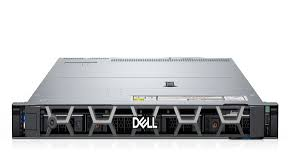
\includegraphics{png/servidorRack.jpeg}
\caption{Figura1: Servidor tipus rack}
\end{figure}

\textbf{Servidor en maxi torre} Son ordinadors de major capacitat de
processament, comunicació per la xarxa local i sistema de redundancia de
dades en els discos durs. Són més usats en organitzacions menys grans.
Tot i que les caixes o torres estan preparades per a ampliacions amb
bahies sobrants i pel seu tamany no ofereixen les facilitats en quan a
escalabilitat dels racks.

\begin{figure}
\centering
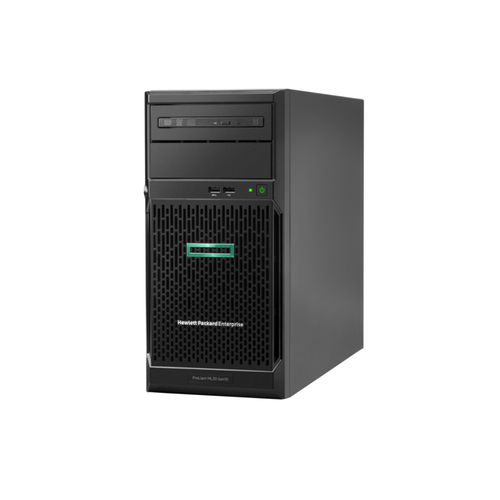
\includegraphics[width=0.5\textwidth,height=\textheight]{png/servidorTorre.jpeg}
\caption{Figura2: Servidor tipus rack}
\end{figure}

\subsubsection{2.2.2 El client}\label{el-client}

El client és el dispositiu o programa que envia peticions al servidor.
Sol ser un ordinador o dispositiu mòbil que permet l'accés als recursos
i serveis proporcionats pel servidor.

\subsubsection{2.2.3 EL Middleware}\label{el-middleware}

És el programari intermediari que facilita la comunicació i la
coordinació entre el client i el servidor.El middleware permet
independitzar els clients i els servidors, sobretot, gràcies als
sistemes oberts, que eliminen la necessitat de supeditar-se a
tecnologies propietàries. Per tant, el middleware facilita el
desenvolupament d' aplicacions, perquè resol la part del transport de
missatges i facilita la interconnexió de sistemes heterogenis sense
utilitzar tecnologies propietàries.

\subsection{2.3 Funcionament bàsic}\label{funcionament-buxe0sic}

El funcionament bàsic es pot resumir en els següents passos:

\begin{enumerate}
\def\labelenumi{\arabic{enumi}.}
\tightlist
\item
  El Servidor espera les sol·lituds.
\item
  El client envia una petició al servidor.
\item
  El servidor processa la petició, fent les comprovacions necessàries i,
  si pertoca\ldots{}
\item
  El servidor respon al client amb la informació o els serveis
  sol·licitats.
\item
  El client fa la comprovació i, si entén que la resposat és correcta la
  mostra al usuari.
\end{enumerate}

A partir d'ací i per l'experiència com a usuaris finals d'un xarxa com
la del IES Maria Enríquez, podem deduir que:

1- El servidor deu estar en marxa abans abans que els clients comencen a
fer sol·licituds. 2- Les sol·licituds son transparents a l'usuari final.
* Accedim a una carpeta del servidor pel GUI o pel CLI com ho fem a una
carpeta local. * Enviem un PDF a una impressora de xarxa com ho fem a
una impressora connectada al nostre USB. 3- Les primeres sol·licituds
que farà tot client estarna relacionades amb: * Autenticar-se en ``la
xarxa'' * Demanar una IP 4- El client podrà tindre o no permís per a
accedir a permisos en funció de qui siga l'usuari, el PC\ldots?

\subsection{2.4 Esquema senzill que
estudiarem}\label{esquema-senzill-que-estudiarem}

El model que emularem amb el VirtualBox per treballar a l'aula i a casa
i també puntualment al taller (si hi ha diponible hores i recursos) serà
un model senzill propis d'una organització simple. Els habituals en
empreses mitjanes o menudes, ajuntaments etc. on tenim un o dos
servidors i unes desenes de PC connectats mitjançant els stwitch.

\begin{figure}
\centering
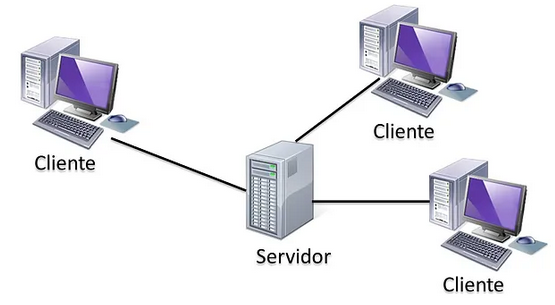
\includegraphics[width=0.7\textwidth,height=\textheight]{png/cs.png}
\caption{Figura 3. Estructura lògica}
\end{figure}

\begin{figure}
\centering
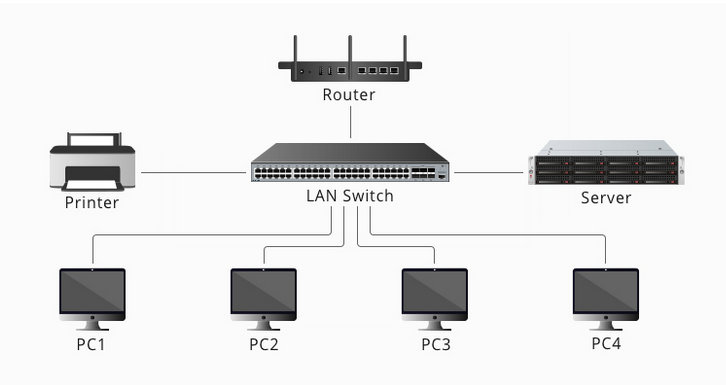
\includegraphics[width=0.7\textwidth,height=\textheight]{png/csXarxaFisica.png}
\caption{Figura 4. Estructura fisica}
\end{figure}

\section{3 Tipus d'arquitectures
Client/Servidor}\label{tipus-darquitectures-clientservidor}

\subsection{3.1 Classificació segons la mida dels costats
(Client/Servidor)}\label{classificaciuxf3-segons-la-mida-dels-costats-clientservidor}

Aquesta classificació es fa en funció de la càrrega que suporta cada
costat de l'arquitectura:

\begin{itemize}
\tightlist
\item
  \textbf{Arquitectura lleugera}: La major part del treball es fa al
  servidor, mentre que el client només presenta els resultats.
\item
  \textbf{Arquitectura pesada}: El client realitza una part important
  del processament, i el servidor actua com a gestor de dades.
\end{itemize}

\subsection{3.2 Segons el tipus de serveis que
ofereix}\label{segons-el-tipus-de-serveis-que-ofereix}

En una arquitectura client-servidor, els serveis proporcionats poden
variar considerablement segons les necessitats de l'empresa o
organització. A continuació, es descriuen alguns dels tipus de serveis
més comuns:

\subsubsection{3.2.1 Servidor de fitxers}\label{servidor-de-fitxers}

Funció: Proporciona emmagatzematge centralitzat per a arxius, que poden
ser accedits, modificats i compartits pels clients de la xarxa.

Ús habitual: Es troba en entorns empresarials on cal compartir
documents, fulls de càlcul, bases de dades o qualsevol altre tipus de
fitxer entre diversos usuaris. Això permet el treball col·laboratiu.

Protocols associats habituals:SMB (Server Message Block) per a entorns
Windows i NFS (Network File System) per a entorns Unix/Linux.

\subsubsection{3.2.2 Servidor de bases de
dades}\label{servidor-de-bases-de-dades}

\textbf{Funció:} Gestiona les bases de dades, processant sol·licituds de
consulta i actualització de dades des dels clients. \textbf{Ús
habitual:} Sistemes de gestió empresarial (ERP), sistemes de comerç
electrònic, o qualsevol aplicació que depenga de dades estructurades.

\textbf{Exemples de software:} MySQL, PostgreSQL, Microsoft SQL Server i
Oracle.

\subsubsection{3.2.3 Ressolució de noms.}\label{ressoluciuxf3-de-noms.}

Sí, la \textbf{resolució de noms} és un \textbf{servei bàsic i
fonamental en les xarxes} que converteix noms de domini i de recursos en
la xarxa en les seus adreces IP, permetent així que els dispositius es
localitzen i es comuniquen entre ells. És essencial per a la navegació
web.

\paragraph{DNS (Domain Name System)}\label{dns-domain-name-system}

El DNS és el servei més conegut per a la resolució de noms. Converteix
noms de domini com \texttt{www.exemple.com} en adreces IP com
\texttt{192.0.2.1}, que els ordinadors utilitzen per comunicar-se entre
ells. Servidors que emmagatzemen i gestionen les dades de noms i
adreces. Inclouen servidors DNS autoritaris, que tenen la informació
definitiva sobre dominis, i servidors DNS recursius, que realitzen
cerques en nom dels clients.

\begin{quote}
Nota: El DNS el vorem prompte en la instal·lació del Windows Server i
l'accès des d'un client Windows 11.
\end{quote}

\paragraph{Hosts File}\label{hosts-file}

Un fitxer de configuració local en els sistemes operatius que mapeja
noms de domini a adreces IP. Els fitxers \texttt{hosts} es poden
utilitzar com a solució temporal per a la resolució de noms en xarxes
petites o per a proves. - \textbf{Ubicació}: - \textbf{Windows}:
\texttt{C:\textbackslash{}Windows\textbackslash{}System32\textbackslash{}drivers\textbackslash{}etc\textbackslash{}hosts}
- \textbf{Linux/Mac}: \texttt{/etc/hosts}

\begin{quote}
Nota: El vorem en configurar el Servidor LDAP de Linux.
\end{quote}

\paragraph{NetBIOS (Network Basic Input/Output
System)}\label{netbios-network-basic-inputoutput-system}

Proporciona un sistema de resolució de noms per a xarxes locals de
Windows. NetBIOS permet que els ordinadors es reconeguin mitjançant noms
en lloc d'adreces IP. - \textbf{Protocols associats}: - \textbf{NBNS
(NetBIOS Name Service)}: Permet la resolució de noms NetBIOS en adreces
IP dins d'una xarxa local.

\begin{quote}
Nota: és el protocol de les xarxes Workgrup menudes sense DNS que vam
vore al curs passat i ara.
\end{quote}

\textbf{Importància del servei de resolució de noms} - \textbf{Facilitat
d'ús}: Permet als usuaris utilitzar noms de domini amigables en lloc
d'adreces IP numèriques, facilitant l'ús i la memòria. -
\textbf{Eficiència}: Redueix la necessitat de memoritzar adreces IP
complexes i facilita l'administració de xarxes mitjançant noms de
domini. - \textbf{Flexibilitat}: Permet actualitzacions i canvis
d'adreces IP sense necessitat que els usuaris final hagin de modificar
les adreces en les seves aplicacions.

En resum, la resolució de noms és un servei fonamental en la
infraestructura de xarxes que facilita la comunicació entre dispositius
i aplicacions mitjançant la traducció de noms humans llegibles en
adreces IP que els sistemes informàtics poden interpretar.

\subsubsection{3.2.5 Servidor web}\label{servidor-web}

Funció: Un servidor web s'encarrega d'allotjar i servir pàgines web als
clients (normalment navegadors web). Aquest servidor interpreta
sol·licituds HTTP enviades pels clients i respon amb els fitxers HTML o
altres recursos necessaris per a renderitzar la pàgina.

Ús habitual: S'utilitza per a llocs web, portals de comerç electrònic i
aplicacions basades en web. Els servidors web són crucials per a l'accés
remot a informació i serveis empresarials.

Protocols associats: HTTP i HTTPS són els protocols principals
utilitzats per als servidors web. Els exemples més comuns de programari
de servidors web són Apache, Nginx i Microsoft IIS.

\subsubsection{3.2.6 Servidor d'autenticació i gestió centralitzada
d'usuaris}\label{servidor-dautenticaciuxf3-i-gestiuxf3-centralitzada-dusuaris}

\textbf{Funció:} La gestió centralitzada d'usuaris permet a les
organitzacions administrar de manera centralitzada les credencials
d'usuari, els permisos i l'accés als recursos compartits en la xarxa. Un
servidor d'autenticació, com Active Directory en entorns Windows o
OpenLDAP en sistemes Linux, centralitza la gestió d'usuaris i controla
qui pot accedir a determinats recursos.

Components clau de la gestió centralitzada d'usuaris

\textbf{Autenticació:} Els usuaris es validen a través d'un sistema
centralitzat abans d'accedir a qualsevol servei. Per exemple, en
sistemes com Active Directory, els usuaris introdueixen un nom d'usuari
i una contrasenya que el servidor verifica.

\textbf{Autorizació:} Una vegada autenticat, el sistema determina els
recursos als quals l'usuari pot accedir segons els seus rols i permisos.
Això permet controlar qui pot visualitzar, modificar o administrar certs
recursos, com ara fitxers o aplicacions.

\textbf{Gestió d'usuaris:} El servidor centralitzat permet afegir,
eliminar o modificar usuaris des d'una ubicació central, la qual cosa
facilita l'administració en grans xarxes amb molts usuaris.

\textbf{Polítiques de seguretat:} Es poden aplicar polítiques de
seguretat uniformes, com ara l'obligatorietat de contrasenyes fortes,
l'expiració periòdica de contrasenyes o l'autenticació multifactor.

Exemples de programari de gestió centralitzada d'usuaris

\textbf{Active Directory (AD):}És la solució de Microsoft per gestionar
usuaris i recursos de xarxa de manera centralitzada en un entorn Windows
Server.

\textbf{LDAP (Lightweight Directory Access Protocol):} Utilitzat sovint
en entorns Unix/Linux per gestionar l'autenticació i permisos a través
d'un directori d'usuaris.

\textbf{Kerberos:} Un protocol d'autenticació de xarxa que utilitza
xifratge de claus simètriques per autenticar els usuaris i serveis dins
d'una xarxa.

La gestió centralitzada d'usuaris és essencial per a qualsevol
organització amb una xarxa corporativa on els usuaris necessiten accedir
a múltiples recursos, com fitxers, aplicacions o serveis. Això permet
que els administradors gestionen permisos i configuracions des d'un únic
punt, millorant l'eficiència i la seguretat.

\subsubsection{3.2.7 Servidor d'impressió}\label{servidor-dimpressiuxf3}

El servidor d'impressió gestiona la impressió de documents en una xarxa,
actuant com a intermediari entre els clients que envien treballs
d'impressió i les impressores disponibles. Això permet als usuaris de la
xarxa enviar els seus documents a una o diverses impressores de forma
centralitzada i organitzada.

Gestió de cues. Els servidors d'impressió poden gestionar la cua
d'impressió, prioritzar les tasques, emmagatzemar temporalment els
documents per a una impressió eficient i controlar l'accés a les
impressores basant-se en permisos d'usuari o grups d'usuaris.

Gestió dels permisos i prioritats. Els administradors poden definir qui
té permís per utilitzar quines impressores, establint polítiques basades
en rols d'usuaris, grups o departaments.

Monitorització i registre d'ús: El servidor pot monitoritzar l'ús de les
impressores i generar informes, permetent als administradors saber qui
està imprimint, la quantitat de pàgines, i controlar l'ús excessiu o no
autoritzat.

Protocols associats: IPP (Internet Printing Protocol): És un dels
protocols més utilitzats per a la comunicació entre clients i servidors
d'impressió. Permet a les aplicacions d'usuari enviar treballs
d'impressió a través d'Internet o d'una xarxa local.

LPD/LPR (Line Printer Daemon/Line Printer Remote): Aquests protocols es
fan servir tradicionalment en entorns Unix/Linux per gestionar les
tasques d'impressió.

SMB (Server Message Block): Utilitzat en entorns Windows, permet
compartir impressores (i fitxers) a través de la xarxa local.

Exemples de programari de servidor d'impressió

Windows Print Server: El servidor d'impressió de Microsoft, integrat en
el sistema operatiu Windows Server, permet gestionar impressores en
xarxa i assignar-les als usuaris de forma centralitzada.

CUPS (Common Unix Printing System): Un programari de codi obert
utilitzat en sistemes Unix/Linux i macOS per gestionar tasques
d'impressió en xarxa.

\subsubsection{3.2.8 Servidor de correu}\label{servidor-de-correu}

Funció: Gestiona el correu electrònic dins de l'organització, tant per a
l'enviament com per a la recepció de missatges. Proporciona serveis com
la gestió de bústies de correu, filtres de correu brossa, i
emmagatzematge d'arxius adjunts.

Ús habitual: Es troba en totes les organitzacions que necessiten
comunicar-se a través del correu electrònic, ja sigui internament o
externament.

Protocols associats: Els protocols més comuns són SMTP (Simple Mail
Transfer Protocol) per a l'enviament de correu, i IMAP (Internet Message
Access Protocol) o POP3 (Post Office Protocol) per a la recepció.

\subsection{3.3 Servidors. Máquines o
serveis?}\label{servidors.-muxe1quines-o-serveis}

Tal com hem exposat la classificació dels servidors segons el servei,
sembla que un Servidor només puga oferir un servei: no es tracta d'això.
De fet, tal i como vorem el mateix Servidor físic fa de servidor de
diversos serveis. Així, direm que el Servidor WIN-SERVER1 ``és el
servidor DNS'' o el ``servidor DHCP'' o el ``servidor d'autenticació a
la xarxa local''. És ``servidor'' aquella màquina que respon a la
petició d'un servei oferint-lo i pot tindre més d'un servei instal·lat i
configurat.

\section{4. Avantatges i inconvenients de l'arquitectura
C/S}\label{avantatges-i-inconvenients-de-larquitectura-cs}

\subsection{4.1. Avantantges}\label{avantantges}

\begin{itemize}
\tightlist
\item
  \textbf{Escalabilitat}: Es pot ampliar afegint més clients o
  servidors.
\item
  \textbf{Seguretat}: Centralització dels recursos amb polítiques de
  seguretat robustes.
\item
  \textbf{Facilitat de manteniment}: El servidor es gestiona de manera
  centralitzada.
\end{itemize}

\subsection{4.2. Inconvenients}\label{inconvenients}

\begin{itemize}
\tightlist
\item
  \textbf{Cost}: Pot ser costós configurar i mantenir els servidors.
\item
  \textbf{Dependència}: Si el servidor falla, els clients poden quedar
  desconnectats.
\end{itemize}

\section{5. L'alternativa a l'arquitectura C/S: els Grups de Treball
(Workgroups)}\label{lalternativa-a-larquitectura-cs-els-grups-de-treball-workgroups}

Els grups de treball (workgroups) són una alternativa al model
client-servidor. En aquests, els recursos es comparteixen directament
entre ordinadors, sense la necessitat d'un servidor centralitzat. Aquest
model és adequat per a xarxes petites, però no s'escalfa bé per a
entorns grans.

Com ja vam vore en el tram final del curs anterior. Un mínim control
assignant permisos senzill d'escriptura o lectura a una carpeta ens
obligava a ``duplicar'' els usuaris en les diferents máquines. El mateix
passava si volíem canviar de màquina, havíem de tindr el nostre usuari
creat en la nova màquina.

EL Workgrup sols és una solució vàlida per a xarxes molt senzilles on es
comparteix pocs recursos o de forma puntual. Qualsevol gestió mínima en
un entorn de treball col·laboratiu i recursos software (Base e dades, pe
exemple) o hardware (impressores, discos\ldots) es complica
excessivament.

\section{6. Sistema operatiu de xarxa
(SOX)}\label{sistema-operatiu-de-xarxa-sox}

\subsection{6.1 Concepte de SOX}\label{concepte-de-sox}

Un \textbf{sistema operatiu de xarxa} és aquell que permet la
comunicació entre diferents ordinadors connectats a una xarxa,
facilitant la gestió centralitzada de recursos com fitxers, aplicacions
o dispositius perifèrics. Alguns exemples són Windows Server, Linux (com
Ubuntu Server) o macOS Server.

\subsection{6.2 Sistemes Operatius de Xarxa més
habituals}\label{sistemes-operatius-de-xarxa-muxe9s-habituals}

Els sistemes operatius més comuns inclouen:

\begin{itemize}
\tightlist
\item
  \textbf{Windows Server}: Popular en entorns empresarials.
\item
  \textbf{Linux (Ubuntu Server, CentOS, etc.)}: Reconegut per la seva
  flexibilitat i codi obert.
\item
  \textbf{macOS Server}: Orientat a entorns creatius.
\end{itemize}

\section{7. Comprovació dels requisists
tècnics}\label{comprovaciuxf3-dels-requisists-tuxe8cnics}

Abans d'instal·lar un sistema operatiu en xarxa, és crucial revisar els
requisits tècnics per assegurar que el maquinari suporta correctament el
sistema. Això inclou revisar la RAM, CPU, espai en disc i compatibilitat
amb dispositius de xarxa.

Aquí tens els requisits mínims actualitzats per als sistemes operatius
més comuns en una infraestructura client-servidor.

\section{8. Requisits dels SOX}\label{requisits-dels-sox}

\subsection{8.1. Per a Windows Server
2019}\label{per-a-windows-server-2019}

Els requisits mínims per instal·lar \textbf{Windows Server 2019} són:

\begin{itemize}
\tightlist
\item
  \textbf{Processador}:

  \begin{itemize}
  \tightlist
  \item
    1.4 GHz de 64 bits
  \end{itemize}
\item
  \textbf{Memòria RAM}:

  \begin{itemize}
  \tightlist
  \item
    \textbf{Mínim}: 512 MB per a instal·lacions de Server Core.
  \item
    \textbf{Recomanat}: 2 GB o més per a la instal·lació amb interfície
    gràfica (\emph{Desktop Experience}).
  \end{itemize}
\item
  \textbf{Disc dur}:

  \begin{itemize}
  \tightlist
  \item
    \textbf{Espai mínim}: 32 GB.
  \item
    \textbf{Espai recomanat}: Més de 40 GB (depèn del rol del servidor).
  \end{itemize}
\item
  \textbf{Altres requisits}:

  \begin{itemize}
  \tightlist
  \item
    Compatible amb \emph{UEFI} 2.3.1c (per a instal·lació segura).
  \item
    Accés a la xarxa per a la instal·lació i activació.
  \end{itemize}
\end{itemize}

\subsection{8.2 Per a Ubuntu Server 22.04
LTS}\label{per-a-ubuntu-server-22.04-lts}

Els requisits per a \textbf{Ubuntu Server 22.04 LTS} són:

\begin{itemize}
\tightlist
\item
  \textbf{Processador}:

  \begin{itemize}
  \tightlist
  \item
    CPU de 1 GHz o superior, compatible amb arquitectura de 64 bits
    (\emph{x86-64} o ARM).
  \end{itemize}
\item
  \textbf{Memòria RAM}:

  \begin{itemize}
  \tightlist
  \item
    \textbf{Mínim}: 512 MB (recomanable 1 GB o més per a millor
    rendiment).
  \end{itemize}
\item
  \textbf{Disc dur}:

  \begin{itemize}
  \tightlist
  \item
    \textbf{Espai mínim}: 2.5 GB per a instal·lació bàsica.
  \item
    \textbf{Espai recomanat}: 10 GB o més, depenent de les aplicacions i
    serveis que es vulguin instal·lar.
  \end{itemize}
\item
  \textbf{Altres requisits}:

  \begin{itemize}
  \tightlist
  \item
    Accés a una connexió de xarxa per a la instal·lació i
    actualitzacions.
  \end{itemize}
\end{itemize}

Aquestes especificacions es recomanen per assegurar un funcionament
mínimament eficient en entorns de producció. Per millors resultats,
\textbf{és recomanable utilitzar més recursos}, especialment quan el
servidor haurà de suportar càrregues pesades o entorns virtualitzats.

\section{9. Elaboració de la documentació sobre instal·lació i
incidències}\label{elaboraciuxf3-de-la-documentaciuxf3-sobre-installaciuxf3-i-inciduxe8ncies}

Una bona pràctica en la gestió de sistemes operatius en xarxa és crear
documentació detallada sobre la instal·lació, configuració i manteniment
dels servidors. Això inclou instruccions pas a pas, captura de
pantalles, diagrames de xarxa i llistats d'incidències amb les solucions
aplicades.

\section{10. La virtualització}\label{la-virtualitzaciuxf3}

La virtualització permet executar múltiples sistemes operatius en una
sola màquina física. Això es fa mitjançant hipervisors, que creen i
gestionen les màquines virtuals. Recordem:

\begin{itemize}
\tightlist
\item
  Hipervisor és el software que permet l'execució de Máquinas Virtuales
  (VM).
\item
  El SO principal sobre el que hem instal·lat l'jipervisor és el sistema
  operatiu amfitrió.
\item
  Els SO de les MV són els SO invitats (guest)
\end{itemize}

Els hipervisors poden ser de 2 tipus:

\begin{itemize}
\item
  \textbf{Tipus 1} Funcionan directamente sobre el hardware. Exemples:
  Promox VE, VMware: ESX / vSphere Hypervisor, Microsoft Hyper-V Server,
  Citrix XenServer, citrix Hypervisor Xen
\item
  \textbf{Tipus 2} Funcionen sobre el SO amfitrió. Exemples: VirtualBox,
  VMWare Workstations/Player, Microsoft Virtual PC, QEMU Virt-Manager
\end{itemize}

\begin{figure}
\centering
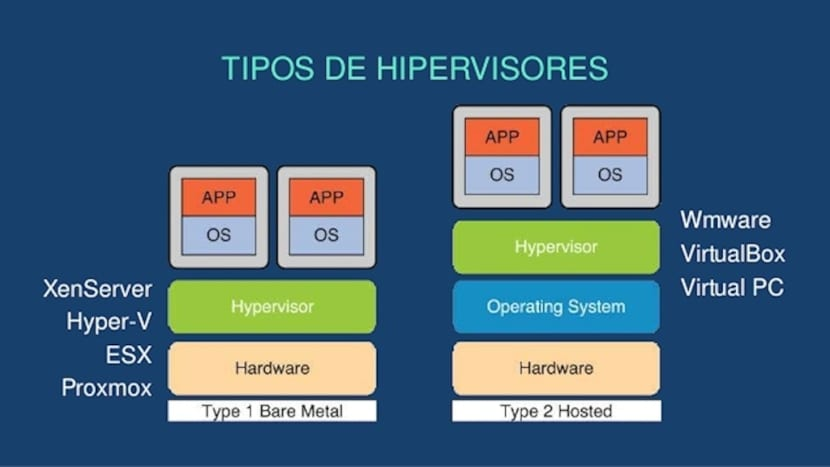
\includegraphics[width=0.75\textwidth,height=\textheight]{png/tiposVirtualizadores.jpg}
\caption{Figura 5. Tipus de Hipervisors}
\end{figure}

\subsection{10.1 Avantatges}\label{avantatges}

\begin{itemize}
\tightlist
\item
  \textbf{Reducció de costos}: Menys maquinari físic.
\item
  \textbf{Flexibilitat}: Facilita la creació de nous entorns de proves o
  producció.
\item
  \textbf{Recuperació ràpida}: Facilita la recuperació davant de
  fallades.
\item
  \textbf{Espais de proves}: Ideal amb finalitat educativa o
  experimental.
\end{itemize}

\subsection{10.2 Ús a l'aula i a casa}\label{uxfas-a-laula-i-a-casa}

Per al mòdul usarem el VirtualBox instal·lant les MV invitadesen un disc
extraïble. D'aquesta manera podrem dur a cas la feina i acabar-la
afegitn la máquina a la instal·lació de VirtualBox que tindrem del curs
passat. Convé revisar que la versió del Hipervisor siga la mateixa.

\begin{figure}
\centering
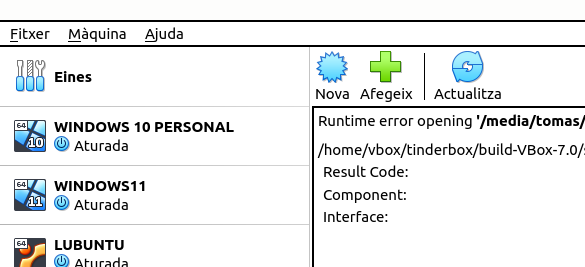
\includegraphics{png/afegeixMV.png}
\caption{Figura 6. Afegir MV a VirtualBox}
\end{figure}

\begin{figure}
\centering
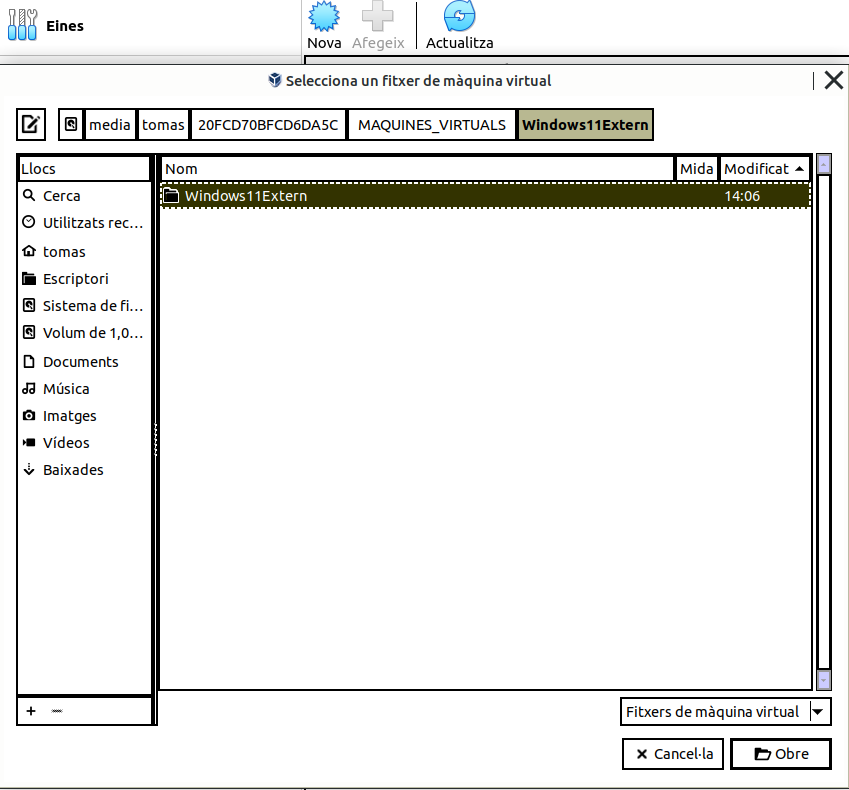
\includegraphics{png/afegeixMV2.png}
\caption{Figura 7. Seleccionar la máquina que tenim al disc extraïble}
\end{figure}

\end{document}
